\chapter{Анализ предметной области}
\label{cha:analysis}
%
% % В начале раздела  можно напомнить его цель
%

В данном разделе будут представлены основные определения, а также будет описана архитектура интернета вещей и поставлена проблема выбора операционной системы для устройств интернета вещей.

\section{Основные определения}

\textbf{Интернет вещей} \cite{Kaspersky} --- это система взаимосвязанных вычислительных устройств, которые могут собирать и передавать данные по беспроводной сети без участия человека. В более широком смысле интернет вещей можно определить как концепцию, описывающую сеть физических объектов ("вещей"), в которые встроены датчики, программное обеспечение и другие технологии для обмена данными с другими устройствами и системами через интернет. \cite{Oracle}

\textbf{Операционная система компьютера} \cite{Olifer} --- комплекс взаимосвязанных программ, который действует как интерфейс между приложениями и пользователями, с одной стороны, и аппаратурой компьютера, с другой стороны.

\textbf{Сетевая операционная система} \cite{Olifer} позволяет пользователю работать со своим компьютером как с автономным и добавляет к этому возможнось доступа к информационным и аппаратным ресурсам других компьютеров сети. В идеальном случае сетевая ОС должна представить пользователю сетевые ресурсы не в виде сети, а в виде ресурсов единой централизованной виртуальной машины. Для такой операционной системы используют специальное название --- \textbf{распределённая ОС}, или \textbf{истинно распределённая ОС}.

Многозадачные ОС подразделяются на три типа в соответствии с использованными при их разработке критериями эффективности:
\begin{itemize}
	\item системы пакетной обработки (OC EC);
	\item системы разделения времени (ОС семейств Linux, Windows, MacOS);
	\item системы реального времени (QNX, FreeRTOS).
\end{itemize}
Современные операционные системы, проектируемые для устройств интернета вещей, являются либо системами реального времени, либо системами разделения времени. \textbf{Операционная система реального времени} \cite{Olifer} --- это система, предназначенная для управления физическими объектами (процессами), которая способна \textit{обеспечить предсказуемое время реакции} в ответ на изменение состояния управляемого объекта (процесса). \textbf{Система разделения времени} \cite{Olifer} --- такая форма организации вычислительного процесса, при которой сразу несколько пользователей одновременно работают на компьютере, причём каждому из них кажется, что он получил компьютер в полное своё распоряжение. Главной целью и критерием эффективности систем разделения времени является \textit{обеспечение удобства и эффективности работы пользователей}.

Ввиду большого многообразия устройств, используемых в распределённых вычислительных системах, при выборе ОС для интернета вещей большую роль играет переносимость. ОС называют \textbf{переносимой} (portable) \cite{Olifer}, или \textbf{мобильной}, если её код может быть сравнительно легко перенесён с процессора одного типа на процессор другого типа и с аппаратной платформы одного типа на аппаратную платформу другого типа. Мобильность - не бинарное состояние, а понятие степени.

Наиболее общим подходом к структуризации операционной системы является разделение всех её модулей на две группы: модули ядра, выполняющие основные функции ОС, и вспомогательные модули ОС. Ядро ОС \cite{Olifer} представляет собой сложный многофункциональный комплекс, имеющий многослойную структуру. В развитии современных операционных систем наблюдается тенденция в сторону переноса кода в верхние слои и удалении при этом всего, что только возможно, из режима ядра, оставляя минимальное \textit{микроядро} \cite{Tanenbaum}. Обычно это осуществляется перекладыванием выполнения большинства задач операционной системы на средства пользовательских процессов. Такой подход способствует переносимости, расширяемости, повышению надёжности системы и создаёт хорошие предпосылки для поддержки распределённых приложений. Модель с микроядром хорошо подходит для поддержки \textbf{распределённых вычислений} \cite{Olifer}, так как использует механизмы, аналогичные сетевым: взаимодействие клиентов и серверов путём обмена сообщениями. Серверы микроядерной ОС могут работать как на одном, так и на разных компьютерах. В этом случае при получении сообщения от приложения микроядро может обработать его самостоятельно и передать локальному серверу или же переслать по сети микроядру, работающему на другом компьютере. Переход к распределённой обработке требует минимальных изменений в работе операционной системы --- просто локальный транспорт заменяется сетевым. В контексте интернета вещей эта концепция приобретает очень большое значение, находя своё применение в разработке распределённых вычислительных систем.

% В \textit{микроядерных} ОС в привилегированном режиме остаётся работать только очень небольшая часть ОС, называемая \textbf{микроядром}. Все остальные высокоуровневые функции ядра оформляются в виде приложений, работающих в пользовательском режиме. Микроядро защищено от остальных частей ОС и приложений. В состав микроядра обычно входят машинно-зависимые модули, а также модули, выполняющие базовые (но не все) функции ядра по управлению процессами, обработке прерываний, управлению виртуальной памятью, пересылке сообщений и управлению устройствами ввода-вывода, связанные с загрузкой или чтением регистров устройств. \cite{Olifer}


\section{Архитектура интернета вещей} 

Определение архитектуры интернета вещей является предметом серьезных дискуссий. 
% Однако все согласны с тем, что для того, чтобы концепция интернета вещей работала, она должна должна состоять из сети, датчиков и коммуникаций. 
Одной из наиболее подробных архитектур является семиуровневая модель, предложенная компанией Cisco \cite{Cisco}. Ниже, в соответствии с рисунком \ref{fig:architecture}, описаны её уровни. \cite{Cisco_architecture_big} \cite{Cisco_architecture_small}

\begin{figure}[h]
	\centering
	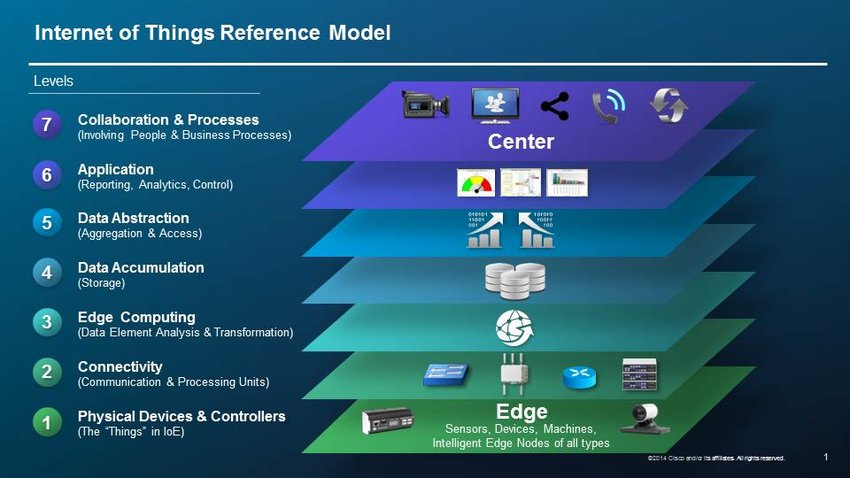
\includegraphics[width=\textwidth ]{img/Illustration-of-the-IoT-Reference-Model-by-Cisco-1.png}
	\caption{Архитектура интернета вещей, предложенная Cisco.}
	\label{fig:architecture}
\end{figure} 

\begin{enumerate}
	\item[1.] \textbf{Физические устройства и контроллеры} --- это уровень, содержащий вещи в IoT. Сюда входит широкий спектр конечных устройств, которые могут отправлять или получать информацию (например, датчики и считыватели радиочастотной идентификации (RFID)).
	\item[2.] \textbf{Соединение} --- это уровень, содержащий все компоненты, способные передавать информацию. Передача может осуществляться между устройствами на первом уровне, между компонентами на этом уровне или между первым и третьим уровнем.
	\item[3.] \textbf{Граничные (туманные) вычисления} --- это первый уровень, на котором происходит обработка данных. Здесь могут собираться и обрабатываться большие объемы информации, что снижает нагрузку на более высокие уровни. Данный уровень также позволяет форматировать и декодировать данные до того, как они будут обработаны.
	\item[4.] \textbf{Накопление данных} --- это уровень, на котором данные сохраняются, чтобы приложения могли получить к ним доступ в случае необходимости. Как правило, необходимая обработка информации не может быть выполнена на сетевых скоростях, поэтому вычислительная система нуждается в промежуточном хранилище данных. Сохранённые данные также могут быть преобразованы и рекомбинированы, чтобы быть готовыми к использованию на более высоких уровнях. В результате на этом уровне данные в движении преобразуются в данные в состоянии покоя.
	\item[5.] \textbf{Абстракция данных} --- это уровень, позволяющий хранить данные более эффективным образом для повышения производительности более высоких уровней. На данном уровне над данными могут выполняться операции нормализации, индексирования, форматирования, проверки, консолидации, а также обеспечивается доступ к нескольким хранилищам данных.
	\item[6.] \textbf{Приложения} --- это уровень, на котором информация, накопленная ранее, интерпретируется приложениями. Именно на этом уровне располагается бизнес-логика приложений.
	\item[7.] \textbf{Взаимодействие и процессы} --- это уровень, объединяющий всё вместе. Система бесполезна, если информация, предоставляемая на этом уровне, не является полезной. Данные из интернета вещей должны использоваться для принятия обоснованных решений.
\end{enumerate}

Операционные системы для интернета вещей существенно упрощают разработку програмного обеспечения для систем с многоуровневой архитектурой, описанной выше, так как позволяют разработчикам абстрагироваться от особенностей аппаратуры конкретных устройств и предоставляют шаблоны для создания приложений с определённой архитектурой.

P.S.: Только попробуйте спросить про единицу измерения простоты! Это не количественная оценка, а КАЧЕСТВЕННАЯ! Здесь может стоять только одно из трёх слов: упрощает, усложняет и не меняет. А упрощает СУЩЕСТВЕННО, потому что ПОЛНОСТЬЮ меняет процесс разработки, а значит, не может влиять в малой степени (тут оценка уже бинарная: меняет либо в большей, либо в меньшей степени).

% Интернет Вещей --- это новая концепция, в которой Интернет эволюционирует от объединения компьютеров и людей к объединению умных вещей.

% Базовой идеей IoT является предоставление возможности автономного обмена полезной информацией между уникально идентифицируемыми объектами реального мира. Эти устройства оснащены новейшими технологиями, такими, как радиочастотная идентификация (RFID) и беспроводные сети датчиков (WSNs), и в дальнейшем получают возможность принимать самостоятельные решения в зависимости от того, какое автоматизированное действие выполняется. 

% Тем не менее, у разных людей и организаций есть свои отличающиеся концепции Интернета Вещей.

% 6-УРОВНЕВАЯ АРХИТЕКТУРА IOT

% Операционные системы устройств интернета вещей (ОСИВ, англ. Internet of Things Operating Systems, IoT OS) позволяют оснащать умные устройства, подключенные к интернету или иной сети связи, основными функциями компьютера с учётом ограниченности вычислительных ресурсов и специфических технических особенностей экосистемы интернета вещей. Такие ОС близки к ранее существовавшему классу операционных систем реального времени (ОСРВ, англ. RTOS)



\section{Проблема выбора операционной системы для интернета вещей}

Операционные системы, предназначенные для интернета вещей, обладают различной функциональностью, которая определяет преимущества и недостатки каждого конкретного решения. Выбранная операционная система должна полностью соответствовать требованиям и ограничениям, предъявляемым к устройствам. Можно выделить четыре основных аспекта и перечень главных вопросов, которые разработчики устройств учитывают при выборе ОС для периферийных устройств IoT. \cite{OS_questions}

% Перед принятием окончательного решения необходимо ответить на четыре основных вопроса.


\begin{enumerate}
	\item[1.] \textbf{Какой уровень надежности и долгосрочной поддержки необходим?} \newline 
	Под надёжностью в данном случае понимается соответствие операционной системы определенным стандартам и сертификациям. Необходимо, чтобы выбранная операционная система обеспечивала варианты, подходящие для конкретных отраслевых стандартов и требований.
	\item[2.] \textbf{Какие требования предъявляются к производительности?} \newline 
	Выбранная операционная система должна соответствовать требованиям устройства к вычислительной мощности и производительности в реальном времени. Также при ответе на данный вопрос стоит учитывать другие аспекты, связанные с производительностью и оказывающие влияние на выбор ОС. К таким можно отнести энергопотребление и объём памяти устройства, а также требования к времени отклика системы на внешние события.
	\item[3.] \textbf{Обеспечивает ли операционная система безопасность устройства?} \newline 
	Безопасность --- один из основных факторов, учитываемых при разработке устройств интернета вещей. Это касается и используемой ОС, так как от неё зависит целостность данных, собираемых устройствами. Если система не обеспечивает необходимый уровень безопасности, то это может привести к порче или краже данных, нарушению запланированных процессов.
	\item[4.] \textbf{Является ли выбранная операционная система масштабируемой?} \newline 
	В связи с тем, что операционные системы, как и любое программное обеспечение, меняются вместе с требованиями к функциям, которые они должны предоставлять. Разработка IoT-устройства с масштабируемой ОС позволяет в будущем адаптироваться к другим задачам без внесения значительных изменений. Масштабируемые ОС могут обрабатывать дополнительные ресурсы без изменения скорости вывода, охватывать несколько устройств и географических регионов.
\end{enumerate}

% Для объединения умных вещей в информационные сети необходимо соответствующее программное обеспечение. Ввиду его сложности ...

% Операционная система - это основная программа IoT-проекта. Современная операционная система Интернета вещей использует технологию облачных вычислений для управления устройствами Интернета вещей в любой точке мира. Благодаря небольшому объему памяти и более высокой эффективности каждая операционная система, представленная ниже, может удовлетворить требования пользователя.




%%% Local Variables:
%%% mode: latex
%%% TeX-master: "rpz"
%%% End:
